\documentclass[border=10pt]{standalone}

\usepackage{tikz}
\usepackage{tikzsymbols}
\usetikzlibrary{calc,patterns,shapes.geometric}

\def\centerarc[#1](#2)(#3:#4:#5){\draw[#1] ($(#2)+({#5*cos(#3)},{#5*sin(#3)})$) arc (#3:#4:#5);}

\begin{document}
	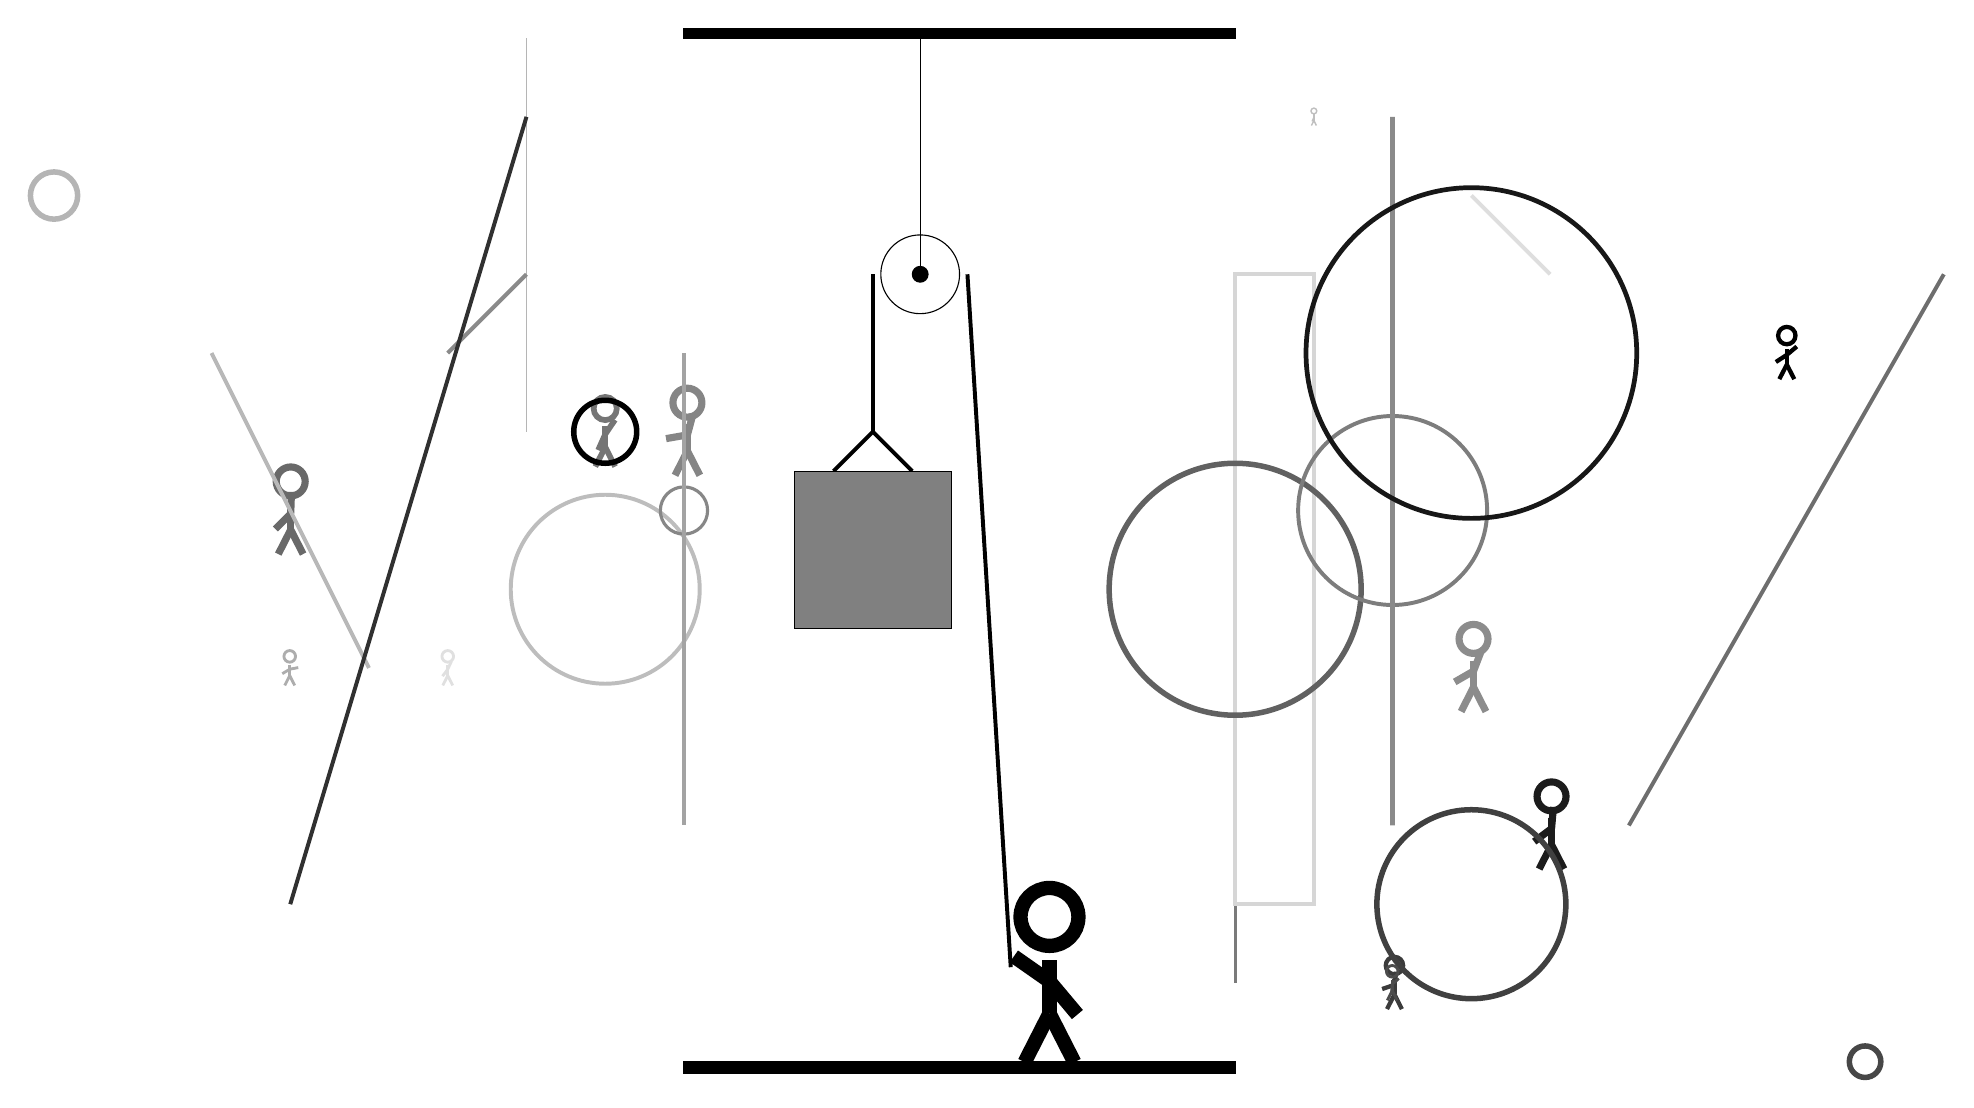
\begin{tikzpicture}
		%%%%% START %%%%%
		
		\draw[fill=black] (-2, 10) rectangle (5, 10.125);
		
		\draw (1, 7) circle (0.5);
		\draw[fill=black] (1, 7) circle (0.1);
		\draw (1, 10) -- (1, 7);
		
		\draw[line width=0.5mm] (-0.1, 4.5) -- (0.4, 5.0) -- (0.9, 4.5);
		\draw[fill=black!50] (-0.6, 4.5) rectangle (1.4, 2.5);
		
		\draw[line width=0.5mm, color=black!57](10, 0) -- (14, 7);
		
		\node[line width=0.7mm, color=black!45] at (8, 2) {\Strichmaxerl[5][30][69]};
		\draw[line width=0.4mm, color=black!52] (5, -2) rectangle (5, 2);
		\node[line width=0.7mm, color=black!12] at (-5, 2) {\Strichmaxerl[2][53][65]};
		\draw[line width=0.6mm, color=black!95] (6, 6) rectangle (6, 2);
		
		\node[line width=0.6mm, color=black!48] at (-2, 5) {\Strichmaxerl[5][10][75]};
		\node[line width=0.5mm, color=black!25] at (6, 9) {\Strichmaxerl[1][66][90]};
		\node[line width=0.5mm, color=black!59] at (-7, 4) {\Strichmaxerl[5][45][88]};
		\draw [line width=0.5mm, color=black!26](-3, 3) circle (1.2);
		\node[line width=0.5mm, color=black!77] at (7, -2) {\Strichmaxerl[3][19][82]};
		\draw[line width=0.2mm, color=black!29] (-4, 10) rectangle (-4, 5);
		
		\node[line width=0.7mm, color=black!54] at (-3, 5) {\Strichmaxerl[4][66][56]};
		\draw [line width=0.4mm, color=black!47](-2, 4) circle (0.3);
		
		\node[line width=0.3mm, color=black!89] at (9, 0) {\Strichmaxerl[5][37][85]};
		\draw [line width=0.7mm, color=black!72](13, -3) circle (0.2);
		\draw[line width=0.5mm, color=black!46](-5, 6) -- (-4, 7);
		
		\draw[line width=0.5mm, color=black!28](-6, 2) -- (-8, 6);
		\draw [line width=0.7mm, color=black!75](8, -1) circle (1.2);
		\draw[line width=0.5mm, color=black!36](-2, 6) -- (-2, 0);
		\draw[line width=0.5mm, color=black!16] (5, 7) rectangle (6, -1);
		\draw [line width=0.7mm, color=black!62](5, 3) circle (1.6);
		
		\draw [line width=0.5mm, color=black!51](7, 4) circle (1.2);
		\draw[line width=0.5mm, color=black!81](-4, 9) -- (-7, -1);
		\draw[line width=0.5mm, color=black!13](8, 8) -- (9, 7);
		\draw [line width=0.7mm, color=black!100](-3, 5) circle (0.4);
		
		\node[line width=0.6mm, color=black!100] at (12, 6) {\Strichmaxerl[3][33][40]};
		\draw[line width=0.6mm, color=black!46] (7, 0) rectangle (7, 9);
		\node[line width=0.5mm, color=black!70] at (7, -2) {\Strichmaxerl[2][86][41]};
		\draw [line width=0.7mm, color=black!29](-10, 8) circle (0.3);
		\draw [line width=0.6mm, color=black!91](8, 6) circle (2.1);
		\node[line width=0.4mm, color=black!32] at (-7, 2) {\Strichmaxerl[2][31][11]};
		
		\draw[line width=0.5mm] (0.4, 7) -- (0.4, 5.0);
		\centerarc[line width=0.5mm](1, 7)(0:180:0.6);
		\draw[line width=0.5mm](1.6, 7) -- (2.15, -1.8);
		
		\node at (2.6, -1.9) {\Strichmaxerl[10][-35][-50]};
		
		\draw[fill=black] (-2, -3) rectangle (5, -3.15);
		
		%%%%% END %%%%%
	\end{tikzpicture}
\end{document}